\section{Components}
The~game server is divided into three separate components. Many instances of a~component can run at~the~same time. Components, and even instances, can be distributed among many machines; this feature renders the~whole server easily scalable. All components internally communicates via HTTP REST API. Refer to Figure \ref{fig:components} for a~component diagram.

\begin{figure}[h]	
	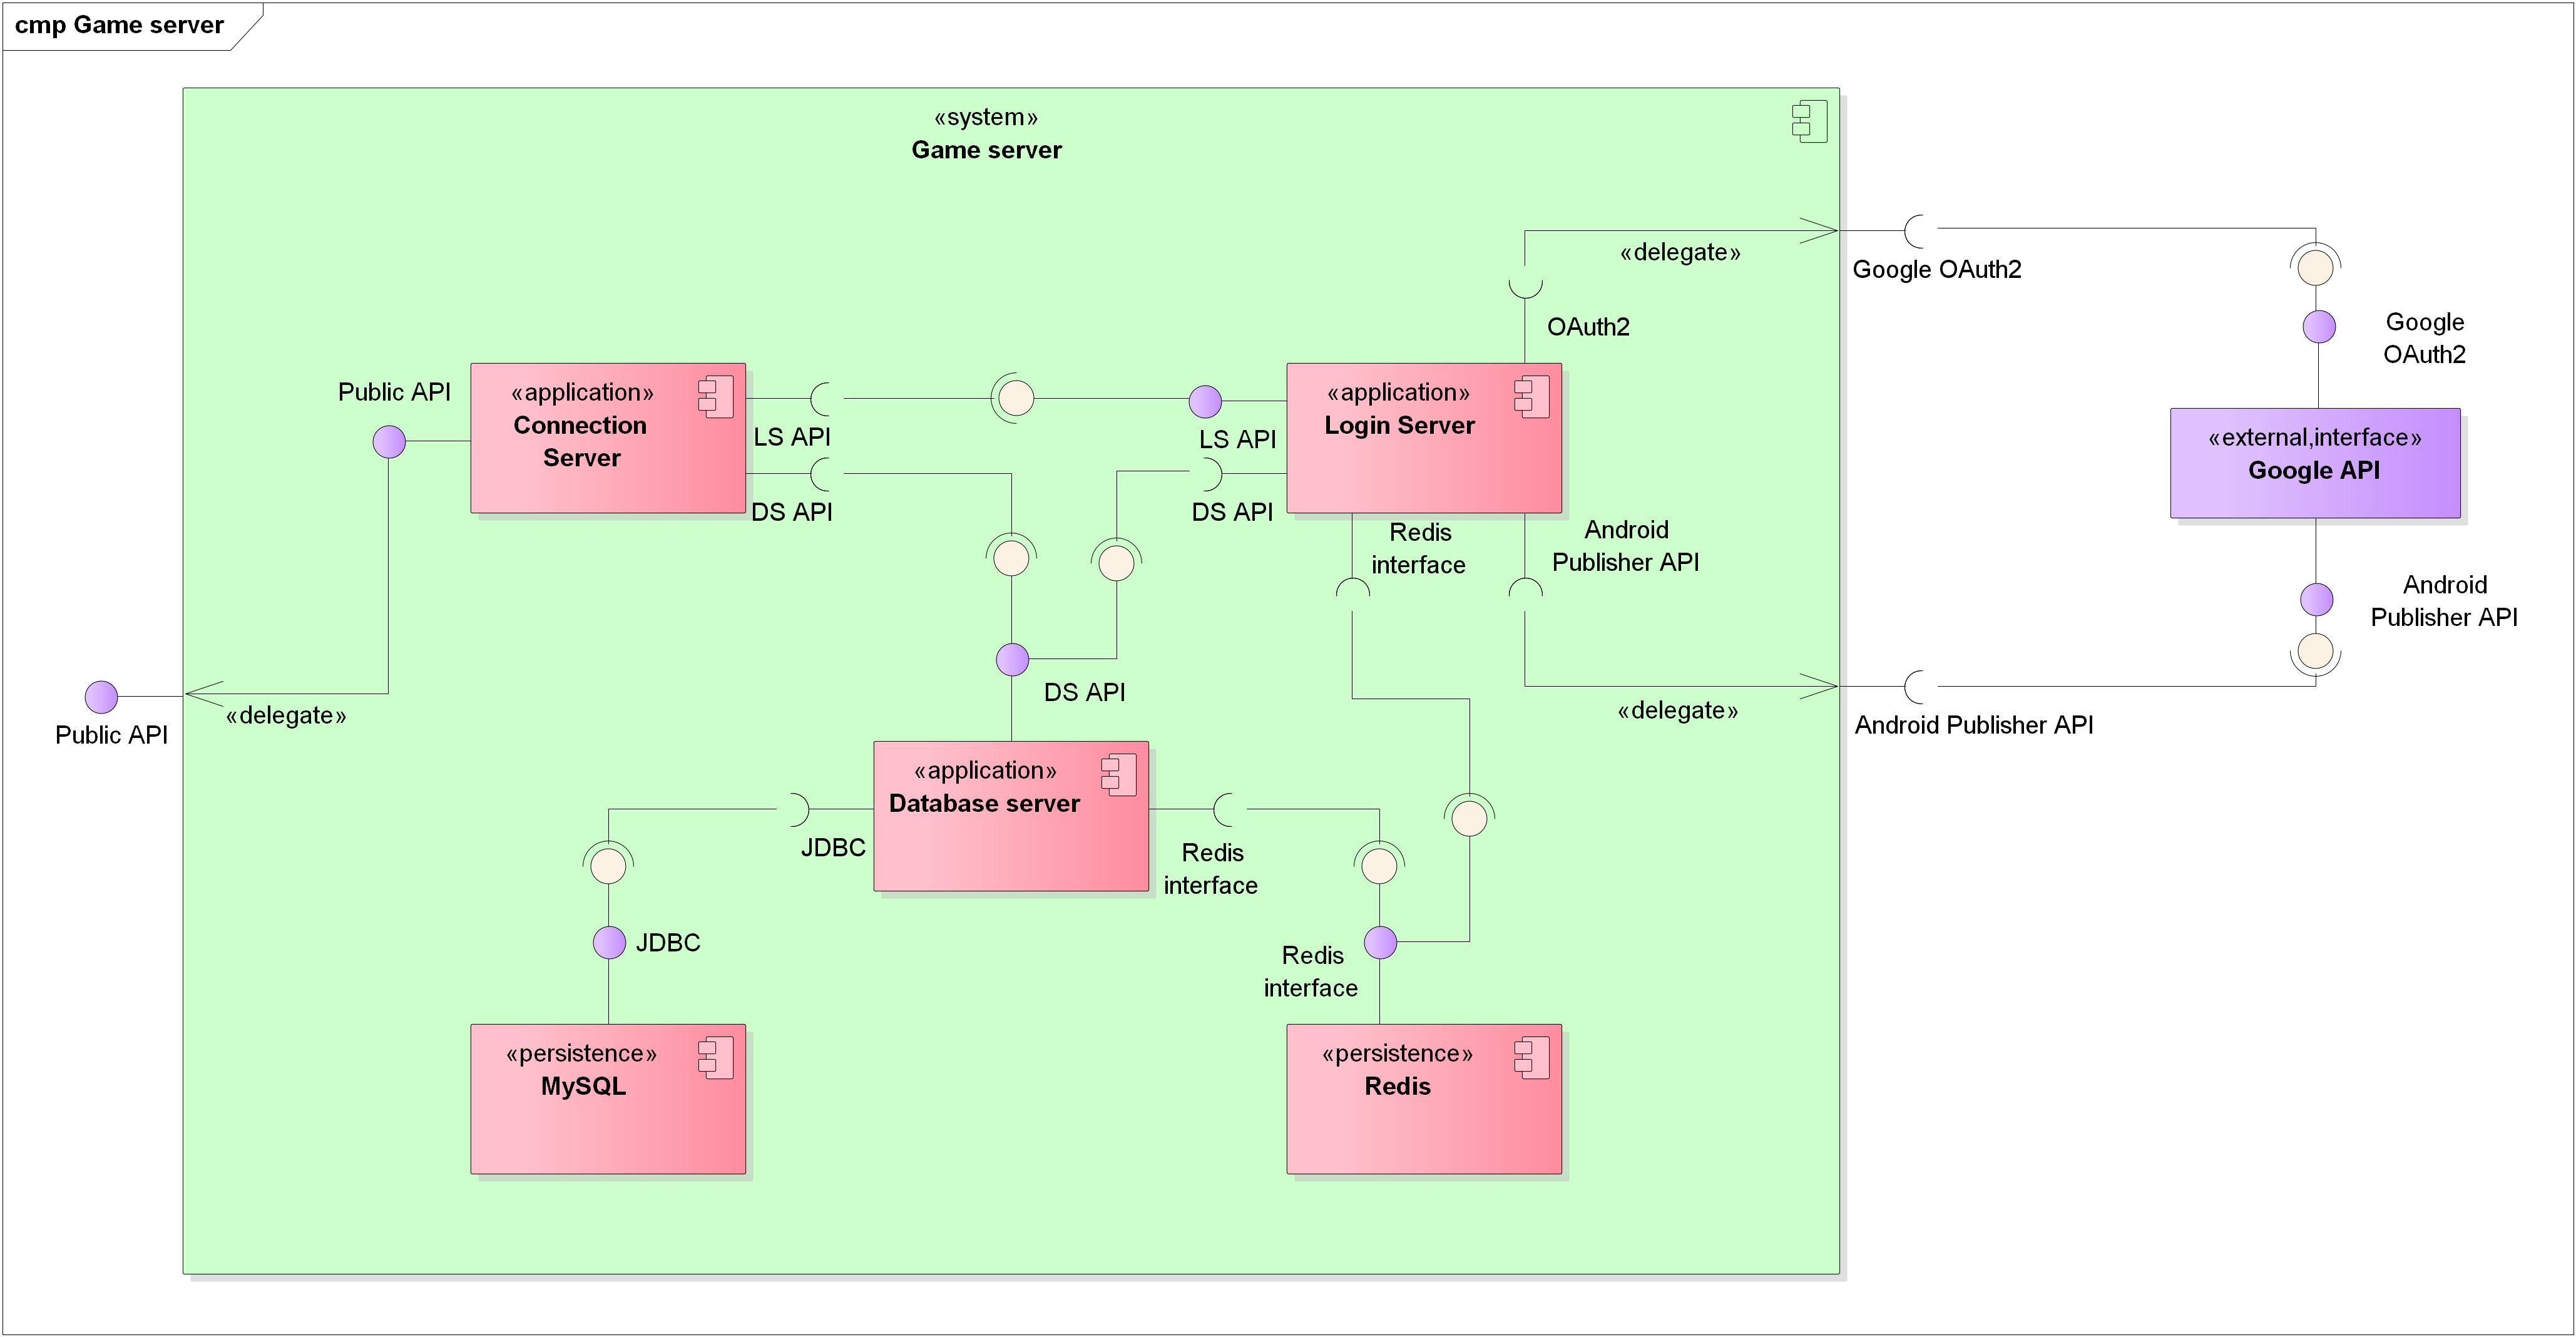
\includegraphics[width=\textwidth]{figures/Components}
	\centering			
	\caption{Component diagram of the~game server}
	\label{fig:components}
\end{figure}

	\subsection{Connection Server}
	This is a~public entry point and the~only component exposed to clients. Reducing the~number of publicly accessible components increases security of the~server. CS handles all incoming traffic and delegates work to other components. 
	
	\subsection{Login Server}
	The~main responsibility of the~LS is to handle user authentication and authorization. It connects to a~Redis server where users' access codes are stored. The~LS is also used for in-app purchase verification. The~component is connected to Google API.
	
	\subsection{Database Server}
	Database server takes care of most of the~game logic. Since the~DS is responsible for data~persistence, it is connected to MySQL and Redis.

\section{Activities}
The following sections describe workflows of actions and activities of clients.
	\subsection{Authentication}
	Authentication process is visualized in Figure \ref{fig:adauth}.
	
	\begin{figure}[h]	
		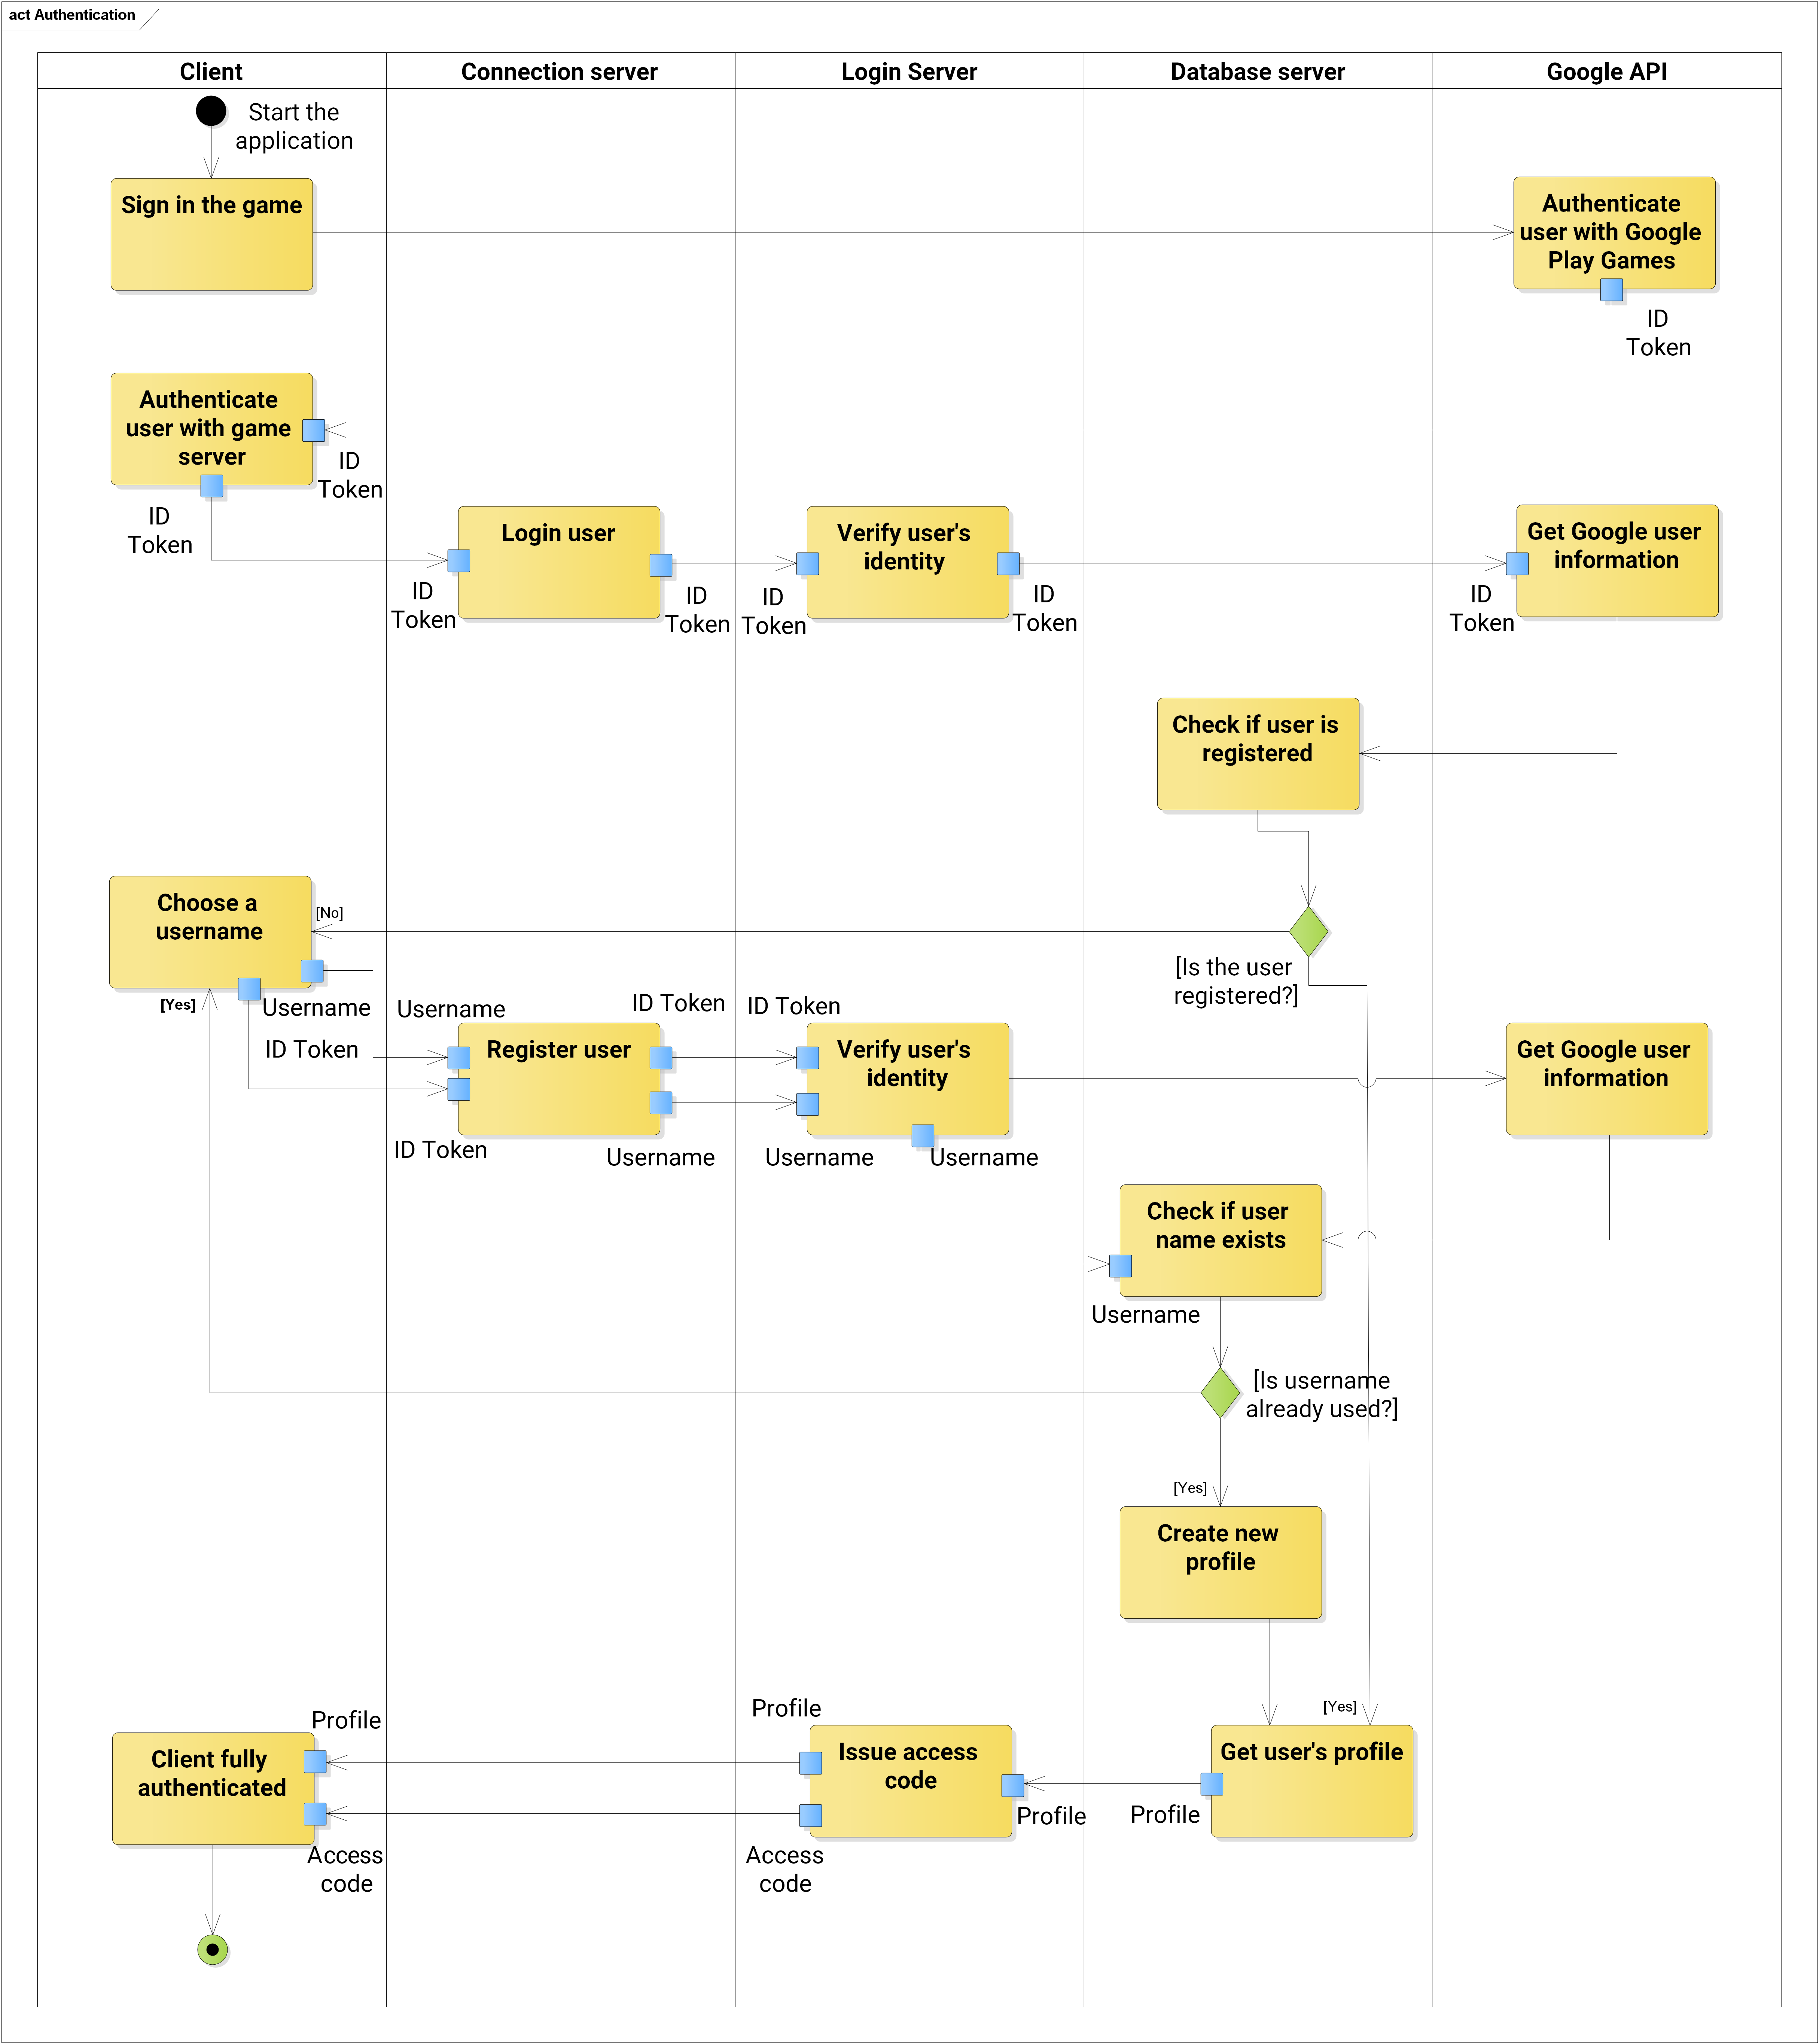
\includegraphics[width=\textwidth]{figures/AD_Authentication2}
		\centering			
		\caption{Activity diagram of the~authentication process}
		\label{fig:adauth}
	\end{figure}

		\subsubsection*{Access Code}
		A~client is identified by his access code during a~session. The~code is random and unique. It is generated each time the~client finishes login process; the~old code,  previously issued to the~user, is invalidated.
		
		\subsubsection*{Registration}
		Every user must register an account to gain access to the~game. The~user is asked to choose a~unique username. If the~username is already taken, the~whole registration process has to be repeated. LS retrieves user's UID and his e-mail address and passes the~information to the~DS, which then creates and initializes a~new user profile. Client is issued an access code and the~authentication process is completed.
		
		\subsubsection*{Login}
		A~registered user can simply login using only his ID Token, which is provided to a~client during login process by Google Play Games. LS exchanges the~token for UID which is then used to retrieve user's profile. Client is issued an access code and the~authentication process is completed.
	
	\subsection{Killing a~Monster}
	A user decides to fight a~monster. In this prototype, the~client iteratively deals damage to the~user and the~monster. The~damage is calculated as \textit{attackDamage} attribute multiplied by a~random value 0.5-1.5. If health of the~monster drops below zero before the~user's one does, the~monster is killed. Server is notified of the~result and rewards the~user with gold and experience. The~kill is logged, the~monster is removed from the~game map and the~client is provided with a~one-time \textit{killConfirmationCode} which allows him to collect loot from the~monster.
		
	\subsection{Killing a~User}
	If user's health drops to or below before the~monster's one does, the~user dies. Client notifies the~server of user's death. His \textit{health} is fully restored and he's punished with \textit{deathPenalty} which is deducted from his gold and scales with his level. See section \ref{section:level} for more details about the~penalty.
	
	\subsection{Collecting Loot after Kill}
	User is presented with an option to collect loot from a~monster he killed. Clients sends a~\textit{killConfirmationCode} along with a~list of items, he wants to collect, to the~server. DS consumes the~\textit{killConfirmationCode} and adds the~selected items to user's inventory. Client then receives the~updated inventory.
	
	\subsection{Buying an Item}
	Client shows its user a~shop and lets him choose what item he wants to buy. The~selected item is sent to the~server. DS verifies the~item is in the~specified shop. Price of the~item is then deducted from user's account and the~item is added to his inventory. If the~user does not have enough gold, the server rejects the~purchase and returns an error message. Otherwise, client receives updated user's inventory.
	
	\subsection{Equipping an Item}
	User selects a~slot and an appropriate item from his inventory. The~client sends the~item along with the~slot to the~server. DS checks if the~item-slot pair is correct and assigns the~item to the~slot. The~successful result is then confirmed to the~client.
	
	\subsection{Using an Item}
	User selects a~usable item from his inventory. Client sends the~selected item to the~server. DS decides what the~item does by looking at attributes \textit{addHealth}, \textit{addExperience}, and \textit{addGold}. Health, experience, and/or gold is added to user's account based on the~values set for the~item. The~updated profile is then sent back to the~client.
		
	\subsection{Purchasing In-app Product}
	In-app purchases are handled client-side which processes the~transactions via a~Google service. The~prototype currently supports only buying gold. If the~transaction is successful, client sends Google's \textit{Purchase token} to the~server. LS verifies the~status of the~purchase using \textbf{Android Publisher API} \cite{androidpublisher} and adds the~gold to user's account. The~purchase is then confirmed to the~client.

	\subsection{Retrieving Nearby Game Objects}
	Client visualizes nearby game objects on the~map. Since the~user moves, the~client frequently retrieves new game objects based on the~actual location, making high demands on the~speed of the~lookup process.
	
	\begin{figure}[h]	
		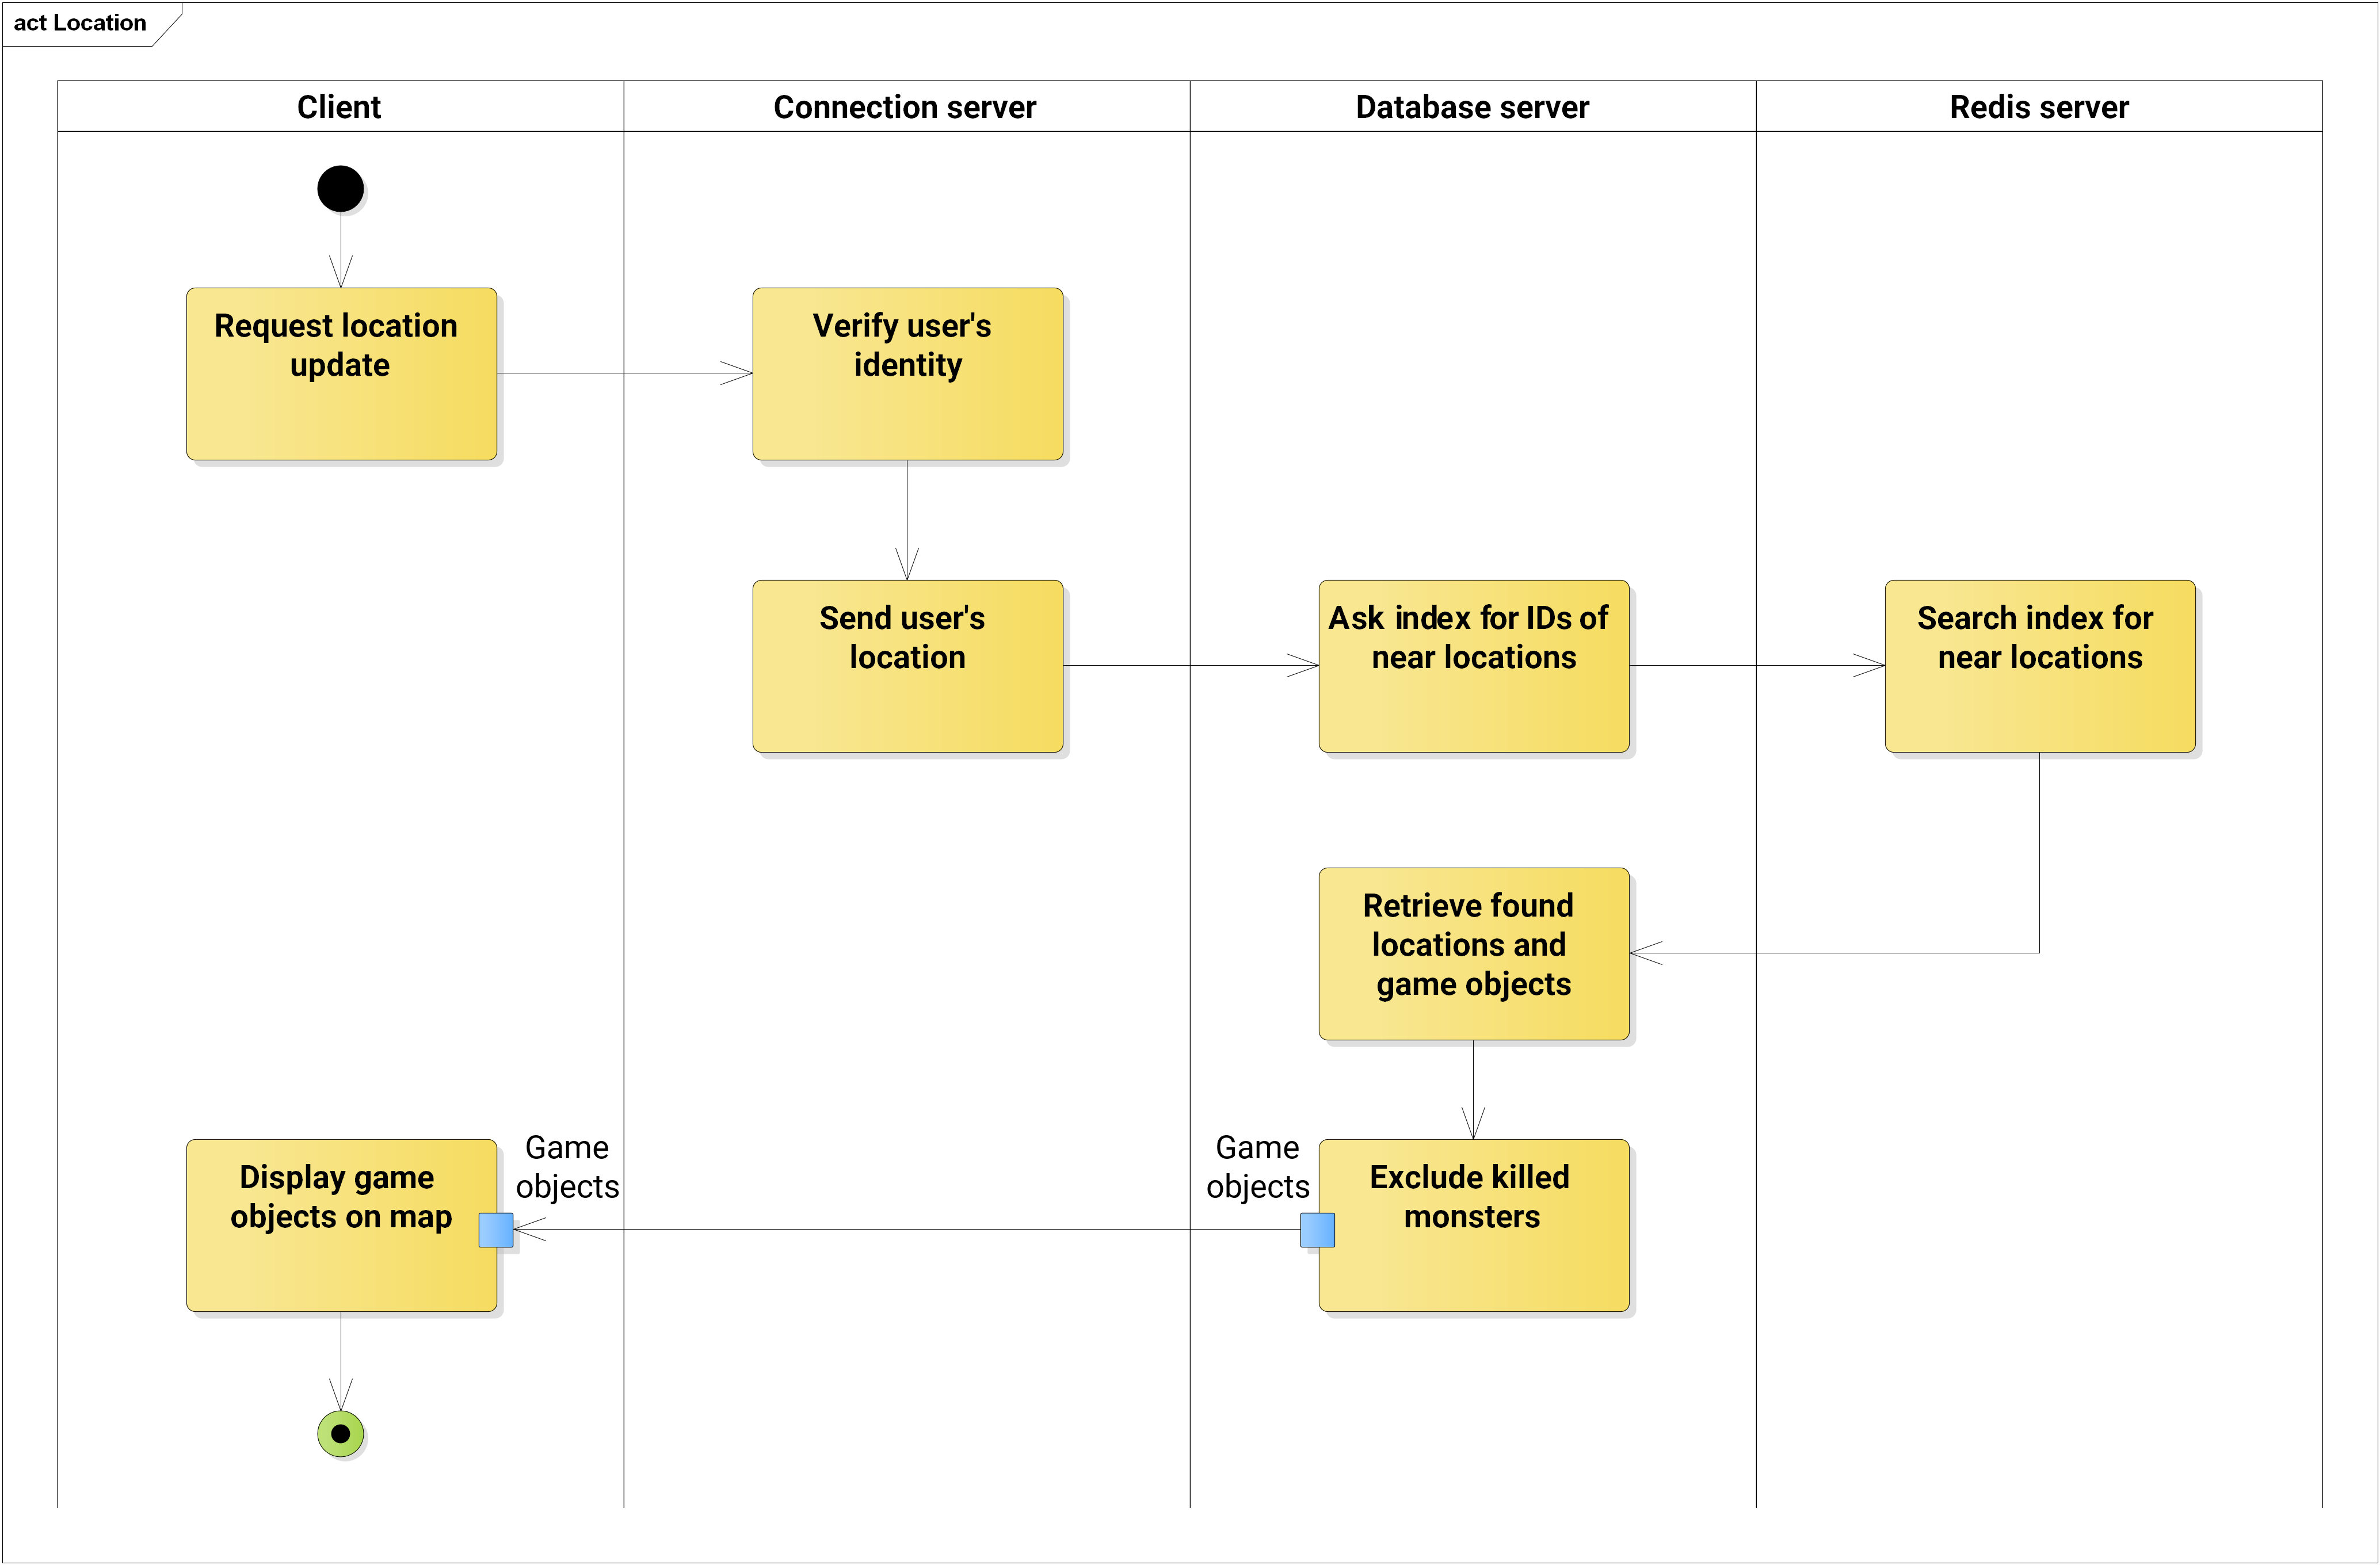
\includegraphics[width=\textwidth]{figures/AD_Location}
		\centering			
		\caption{Activity diagram visualizing how the~server provides nearby game objects}
		\label{fig:adlocation}
	\end{figure} 
	
	Client sends its coordinates to the~server. DS queries Redis which contains an index of all available locations. The~index responds with IDs of locations in 200 m radius from the~provided coordinates. The~locations and their assigned locations are then retrieved from the~database. Server excludes already killed monsters. The~list of locations and their locations is sent to the~client which presents them on the~map. See the~activity diagram of the~described process in Figure~\ref{fig:adlocation}.		

\section{Database Model}
	The database was designed to comply with the~requirements specified in section \ref{section:requirements}. The~entire database model is shown in Figure \ref{fig:dbmodel}. In the~following text, I will describe important tables.	
	
	\begin{figure}[h]	
		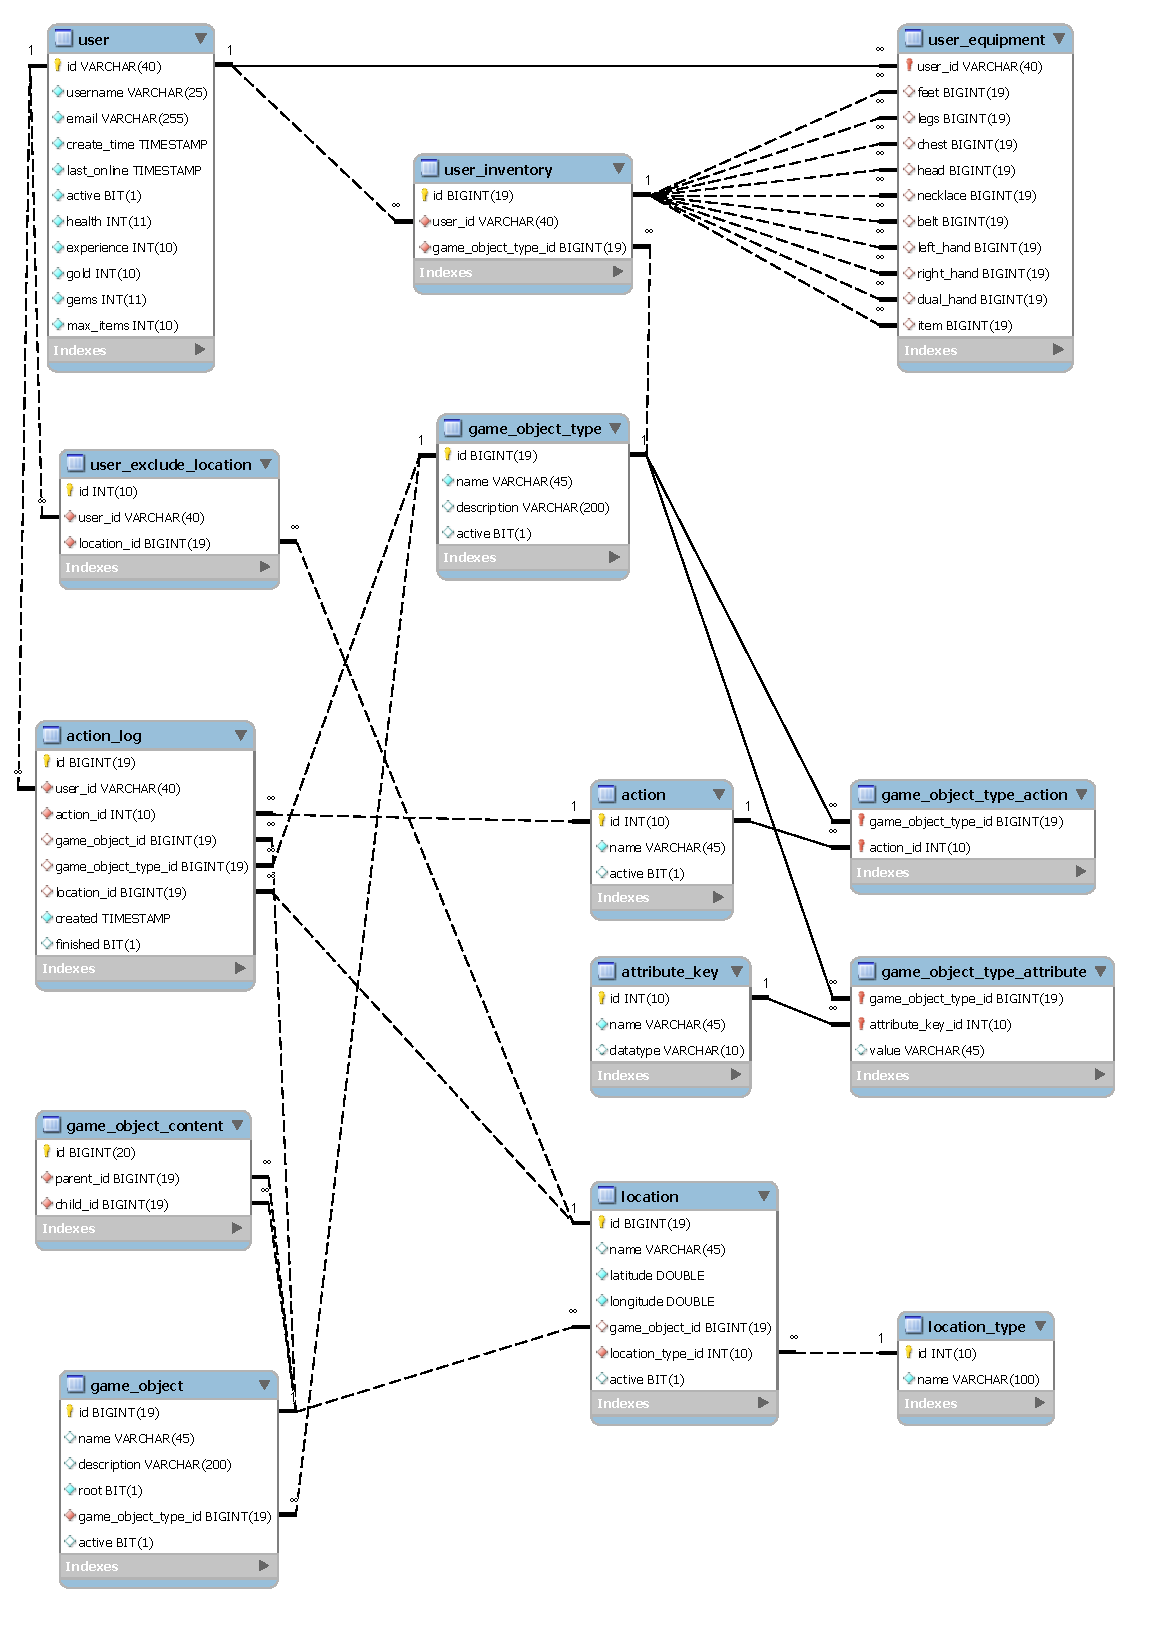
\includegraphics[width=\textwidth]{figures/DatabaseModel}
		\centering
		\caption{Database model}
		\label{fig:dbmodel}	
	\end{figure}
	
	\begin{description}
		\item[user] User's profile. It contains e-mail, UID, and username. Quality attributes of the~profile are also stored here -- current health, experience, and gold.
		
		\item[user\_inventory] Items a~user own. 
		
		\item[user\_equipment] Information about what items a~user has equipped. The~table is in 1:1 relationship with \textit{user}. Each column represents an equipment slot. Server links the~entries in \textit{user\_inventory} to slots in \textit{user\_equipment} to remember equipped items.
		
		\item[game\_object\_type] A ``recipe" for every object in the~game. Name and description of an object are stored here. The~\textit{game\_object\_type} owns attributes and actions.
	
		\item[action] Defines all allowed actions. Each game object type links to a~subset of the~actions.
		
		\item[game\_object\_type\_attribute] Defines all attributes of a~game object. The~attribute is identified by its name and can have a~value.
	
		\item[game\_object] An more concrete definition of a~game object type which can be assigned to a~location.
	
		\item[game\_object\_content] Inventory of a~game object.
	
		\item[location] Predefined real-world locations. Each one must define valid latitude and longitude; location can have a~game object assigned. 
	
		\item[action\_log] Log of user's actions. In prototype, it is used only for kills to allow collecting loot.

		\item[user\_exclude\_location] Locations at which a~user killed a~monster. The~table is periodically flushed. 
		
	\end{description}

\section{Administration}
The Database server supports several API endpoints through which authorized administrators can manage the~game data. The~\textit{Admin} section is protected using \textit{HTTP Basic Authentication} and thus the~administrator has to know a~valid username-password combination. For prototyping purposes, I've decided to provide only basic functionality for the~administration.

	\subsection{Front-end Design}
	Administrators can use a~web front-end to manage game objects, their types, and locations. All actions are accessible from top-side menu. 
	
	For example, when there's a~need to update inventory of an existing game object, it is possible to use the~interface from Figure \ref{fig:wireframegameobject}. After selecting a~game object, the~website presents administrator with two panes, first of which displays all available objects and the~second one shows current inventory of the~selected game object. New items can be added to the~inventory by simply selecting an item from the~first list and then clicking a~\textbf{>>} button
	
	\begin{figure}[h]	
		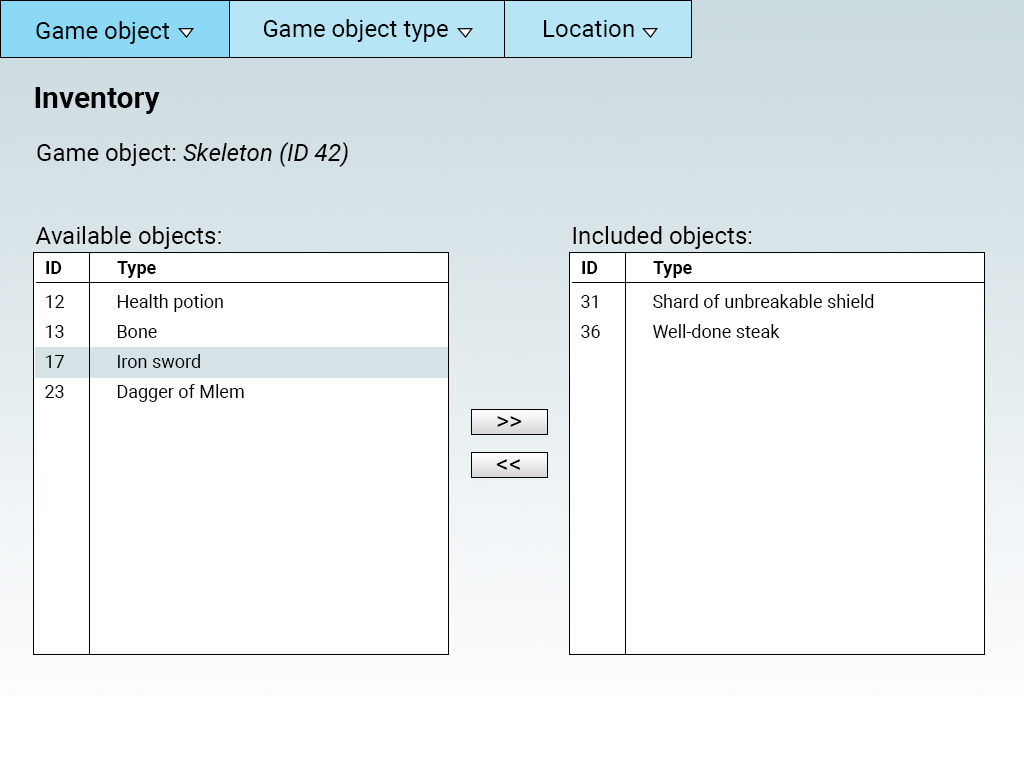
\includegraphics[width=\textwidth]{figures/GameObjectAdminWireframe}
		\centering			
		\caption{Wire-frame of administration front-end - game object inventory}
		\label{fig:wireframegameobject}
	\end{figure}	
	
	The front-end won't be implemented during the~prototyping phase. Administrators can directly call API endpoints to manage game data.	

	\subsection{Game Object Type Management}
	Endpoint \textit{/admin/gameObjectType} alows administrators to create, update and get game object types. Sending a~POST request to the~endpoint will result in a~new game object. A unique name must be specified for the~new type. Optionally, the~type can include a~description, a~set of allowed actions and a~list of attributes.
	
	PUT request updates an existing game object type. It is possible to change name and description. Administrator can also add new attributes and actions. 
		
	All existing game object types can be retrieved along with their actions and attributes by passing a~GET request to the~endpoint.
	
	\subsection{Game Object Management}
	Similarly to their types, game objects themselves can be created, updated and retrieved via endpoint \textit{/admin/gameObject}. Administrator can create new game objects by sending a~POST requests to the~mentioned endpoint. Game object type must be specified for the~new game object. Optionally, the~new object can have an inventory. Even though the~inventory can be filled up during the~creation process, server offers a~PUT method on the~endpoint which replaces the~current children with the~ones in the~request.
	
	All existing game objects can be retrieved along with their children by passing a~GET request to the~endpoint.
	
	\subsection{Location Import}
	New locations can be imported from a~file in OSM XML format \cite{osmxml}. Administrator can do so via a~POST request to \textit{/admin/importLocations}. The~file is parsed for latitude and longitude data and the~new locations are inserted into the~database.
	
	\subsection{Game Object To a~Location Assignment}
	A location serves no purpose without a~\textit{game object} assigned. This can be achieved using PUT endpoint 
	\textit{/admin/assignGameObjectToLocation}.
	
	\subsection{Cache Clearing}
	Developers might need to change game data directly in the~database. Since Hibernate won't be aware of such changes, its cache must be cleared via DELETE endpoint \textit{/admin/clearCache}.
	
\section{Calculations}
Following sections describe how player's level, maximum health and death penalty scales throughout the~game. The~values were chosen experimentally with respect to the~currently implemented game objects. Actual values might and probably will change when new game objects are added.

	\subsection{Level}
	\label{section:level}
	A player gains experience as he progresses the~game. The~amount of experience needed for next level increases with golden ratio. The~game uses the~following formula to calculate player's level from his total experience: 
	\[ level = \left\lfloor{\left(\frac{xp}{1024}\right)^{0.62} + 1}\right\rfloor, \]
	where $xp$ is user's experience.
	\subsection{Maximum Health}
	Player's maximum linearly scales with his level which results in easier fights with strong monsters at higher levels.
	\[ maxHealth = 200 + 50 * (userLevel - 1) \]
	
	\subsection{Death Penalty}
	A player is punished by losing gold when he dies. The~total amount of the~lost gold scales with user's level.
	\[ deathPenalty = 200 + 100 * (userLevel - 1) \]

\section{Public API}
Even though every component has its own API, only the~Connection Server API is available to clients. HTTP methods correspond to REST principles.

The~public API for the~prototype has been specified in cooperation with my colleague Tomáš Zahálka. I present an example of two endpoints below. For the~full list of publicly available API endpoints, please refer to Appendix~\ref{appendix:api}. The~mentioned appendix also contains description of API provided by LS and DS. 	

	\subsection{GET /login}
		The Login endpoint verifies a~Google ID access code and generates an access code for future request. When successfully authenticated, user's profile and the~access code is returned.
		\paragraph*{Parameters}
		\begin{description}
			\item[token] Google ID token [string]
		\end{description}
		\paragraph*{Responses}
		\begin{description}
			\item[200] User successfully logged in, return \textbf{Profile} (\ref{json:profile}) with access code set.
			\item[403] Invalid access code
			\item[404] User not found
			\item[500] Unexpected error
		\end{description}
	
	\subsection{GET /location}
		The Location endpoint retrieves all nearby locations in radius 200 m from the~provided coordinates. The~locations are returned along with their associated game objects.
		\paragraph*{Parameters}
		\begin{description}
			\item[accessCode] Access code [string]
			\item[lat] Latitude [double]
			\item[lon] Longitude [double]
		\end{description}
		\paragraph*{Responses}
		\begin{description}
			\item[200] Return list of nearby \textbf{Location} objects (\ref{json:location}) along with their assigned \textit{game object}.
			\item[403] Invalid access code
			\item[404] User not found
			\item[500] Unexpected error
		\end{description}